\chapter{补充更多细节}

\section{补充图}

\subsection{补充图}

这是附录内容,应该用宋体小四号字体。

\begin{figure}[h!]
	\centering
	\makebox[0.16\textwidth]{\scriptsize 图像}
	\makebox[0.16\textwidth]{\scriptsize 真值}
	\makebox[0.16\textwidth]{\scriptsize Grid-5LSTM1}
	\makebox[0.16\textwidth]{\scriptsize Grid-5LSTM3}
	\makebox[0.16\textwidth]{\scriptsize Grid-5LSTM5} \\
	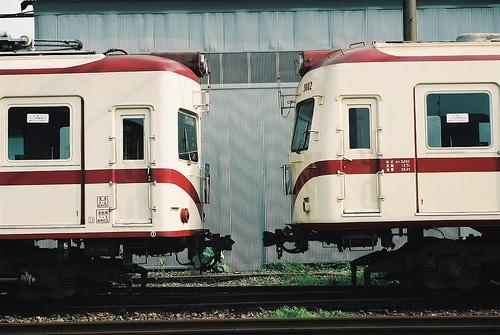
\includegraphics[width=0.16\textwidth]{image/appendix1/2007_000042.jpg}
	
\includegraphics[width=0.16\textwidth]{image/appendix1/2007_000042.png}
	
\includegraphics[width=0.16\textwidth]{image/appendix1/1/2007_000042.png}
	
\includegraphics[width=0.16\textwidth]{image/appendix1/3/2007_000042.png}
	
\includegraphics[width=0.16\textwidth]{image/appendix1/5/2007_000042.png} \\

	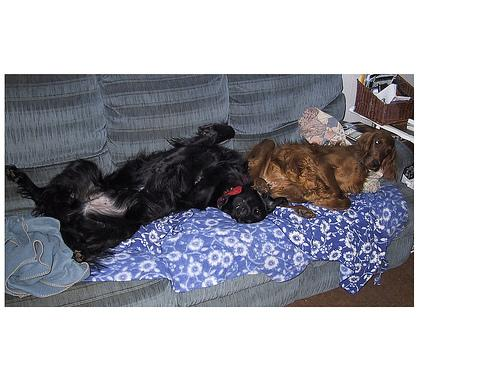
\includegraphics[width=0.16\textwidth]{image/appendix1/2011_003256.jpg}
	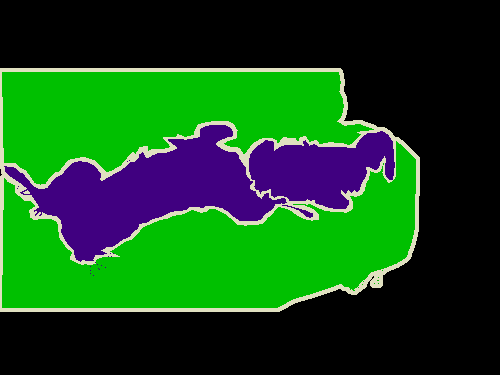
\includegraphics[width=0.16\textwidth]{image/appendix1/2011_003256.png}
	
\includegraphics[width=0.16\textwidth]{image/appendix1/1/2011_003256.png}
	
\includegraphics[width=0.16\textwidth]{image/appendix1/3/2011_003256.png}
	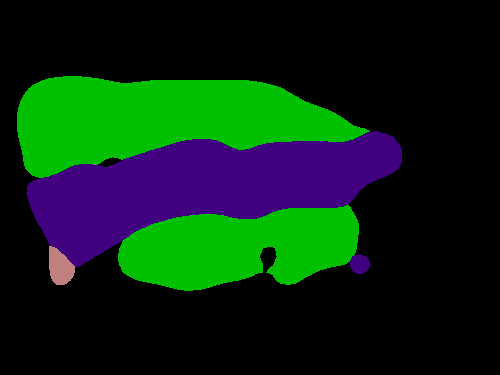
\includegraphics[width=0.16\textwidth]{image/appendix1/5/2011_003256.png} \\
	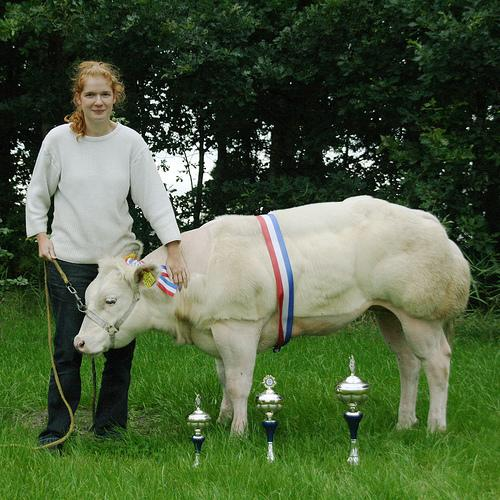
\includegraphics[width=0.16\textwidth]{image/appendix1/2011_001159.jpg}
	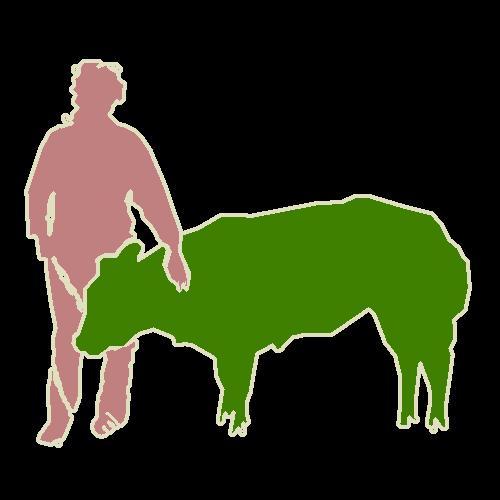
\includegraphics[width=0.16\textwidth]{image/appendix1/2011_001159.png}
	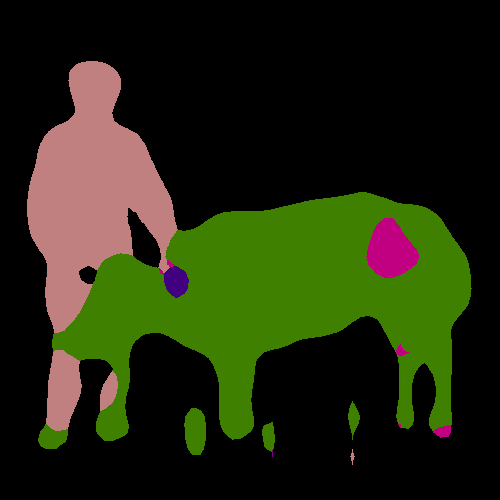
\includegraphics[width=0.16\textwidth]{image/appendix1/1/2011_001159.png}
	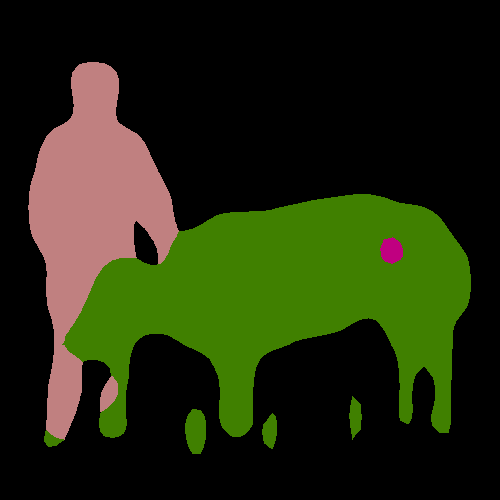
\includegraphics[width=0.16\textwidth]{image/appendix1/3/2011_001159.png}
	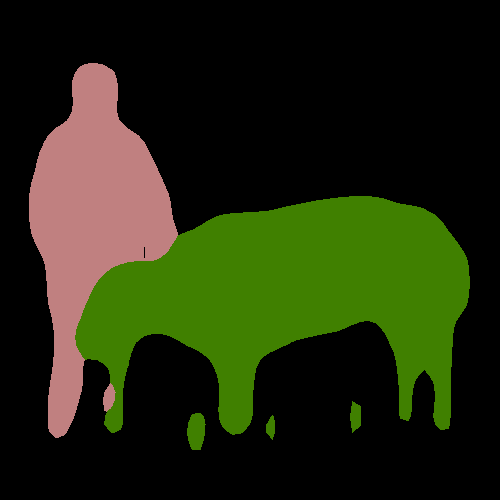
\includegraphics[width=0.16\textwidth]{image/appendix1/5/2011_001159.png} \\
	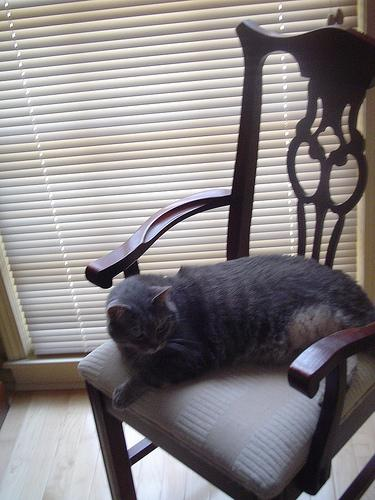
\includegraphics[width=0.16\textwidth]{image/appendix1/2011_000813.jpg}
	
\includegraphics[width=0.16\textwidth]{image/appendix1/2011_000813.png}
	
\includegraphics[width=0.16\textwidth]{image/appendix1/1/2011_000813.png}
	
\includegraphics[width=0.16\textwidth]{image/appendix1/3/2011_000813.png}
	
\includegraphics[width=0.16\textwidth]{image/appendix1/5/2011_000813.png} \\
	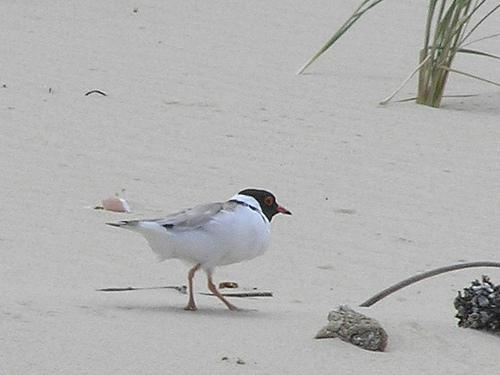
\includegraphics[width=0.16\textwidth]{image/appendix1/2011_003145.jpg}
	
\includegraphics[width=0.16\textwidth]{image/appendix1/2011_003145.png}
	
\includegraphics[width=0.16\textwidth]{image/appendix1/1/2011_003145.png}
	
\includegraphics[width=0.16\textwidth]{image/appendix1/3/2011_003145.png}
	
\includegraphics[width=0.16\textwidth]{image/appendix1/5/2011_003145.png} \\
	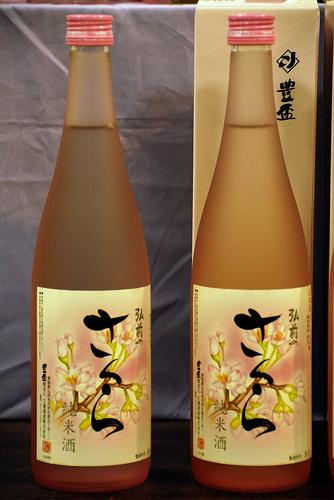
\includegraphics[width=0.16\textwidth]{image/appendix1/2009_004579.jpg}
	
\includegraphics[width=0.16\textwidth]{image/appendix1/2009_004579.png}
	
\includegraphics[width=0.16\textwidth]{image/appendix1/1/2009_004579.png}
	
\includegraphics[width=0.16\textwidth]{image/appendix1/3/2009_004579.png}
	
\includegraphics[width=0.16\textwidth]{image/appendix1/5/2009_004579.png} \\
	\color[rgb]{0.9,0.9,0.9}\bfseries
	\begin{tabular}{*{7}{>{\centering\arraybackslash}p{0.10\textwidth}}}
		\hline
		\cellcolor[rgb]{0,0,0}  背景                 & \cellcolor[rgb]{0.5020,0,0} 飞机         & \cellcolor[rgb]{0,0.5020,0} 自行车 & \cellcolor[rgb]{0.5020,0.5020,0} 鸟 & \cellcolor[rgb]{0,0,0.5020} 船        & \cellcolor[rgb]{0.5020,0,0.5020} 瓶子 & \cellcolor[rgb]{0,0.5020,0.5020} 大巴
		\\
		\hline
		\cellcolor[rgb]{0.5020,0.5020,0.5020} 汽车   & \cellcolor[rgb]{0.2510,0,0} 猫           & \cellcolor[rgb]{0.7529,0,0} 椅子   & \cellcolor[rgb]{0.2510,0.5020,0} 牛 & \cellcolor[rgb]{0.7529,0.5020,0} 桌子 & \cellcolor[rgb]{0.2510,0,0.5020} 狗   & \cellcolor[rgb]{0.7529,0,0.5020} 马   \\
		\hline
		\cellcolor[rgb]{0.2510,0.5020,0.5020} 摩托车 & \cellcolor[rgb]{0.7529,0.5020,0.5020} 人 & \cellcolor[rgb]{0,0.2510,0} 盆栽   & \cellcolor[rgb]{0.5020,0.2510,0} 羊 & \cellcolor[rgb]{0,0.7529,0} 沙发      & \cellcolor[rgb]{0.5020,0.7529,0} 火车 & \cellcolor[rgb]{0,0.2510,0.5020} 电视 \\
		\hline
	\end{tabular}

	\caption{一个配有彩色表格的插图}
\end{figure}

\endinput
